\documentclass[]{article}
\usepackage{lmodern}
\usepackage{amssymb,amsmath}
\usepackage{ifxetex,ifluatex}
\usepackage{fixltx2e} % provides \textsubscript
\ifnum 0\ifxetex 1\fi\ifluatex 1\fi=0 % if pdftex
  \usepackage[T1]{fontenc}
  \usepackage[utf8]{inputenc}
\else % if luatex or xelatex
  \ifxetex
    \usepackage{mathspec}
  \else
    \usepackage{fontspec}
  \fi
  \defaultfontfeatures{Ligatures=TeX,Scale=MatchLowercase}
\fi
% use upquote if available, for straight quotes in verbatim environments
\IfFileExists{upquote.sty}{\usepackage{upquote}}{}
% use microtype if available
\IfFileExists{microtype.sty}{%
\usepackage{microtype}
\UseMicrotypeSet[protrusion]{basicmath} % disable protrusion for tt fonts
}{}
\usepackage[margin=1in]{geometry}
\usepackage{hyperref}
\hypersetup{unicode=true,
            pdftitle={Supervised Learning II Notes},
            pdfauthor={Shivam Verma},
            pdfborder={0 0 0},
            breaklinks=true}
\urlstyle{same}  % don't use monospace font for urls
\usepackage{color}
\usepackage{fancyvrb}
\newcommand{\VerbBar}{|}
\newcommand{\VERB}{\Verb[commandchars=\\\{\}]}
\DefineVerbatimEnvironment{Highlighting}{Verbatim}{commandchars=\\\{\}}
% Add ',fontsize=\small' for more characters per line
\usepackage{framed}
\definecolor{shadecolor}{RGB}{248,248,248}
\newenvironment{Shaded}{\begin{snugshade}}{\end{snugshade}}
\newcommand{\AlertTok}[1]{\textcolor[rgb]{0.94,0.16,0.16}{#1}}
\newcommand{\AnnotationTok}[1]{\textcolor[rgb]{0.56,0.35,0.01}{\textbf{\textit{#1}}}}
\newcommand{\AttributeTok}[1]{\textcolor[rgb]{0.77,0.63,0.00}{#1}}
\newcommand{\BaseNTok}[1]{\textcolor[rgb]{0.00,0.00,0.81}{#1}}
\newcommand{\BuiltInTok}[1]{#1}
\newcommand{\CharTok}[1]{\textcolor[rgb]{0.31,0.60,0.02}{#1}}
\newcommand{\CommentTok}[1]{\textcolor[rgb]{0.56,0.35,0.01}{\textit{#1}}}
\newcommand{\CommentVarTok}[1]{\textcolor[rgb]{0.56,0.35,0.01}{\textbf{\textit{#1}}}}
\newcommand{\ConstantTok}[1]{\textcolor[rgb]{0.00,0.00,0.00}{#1}}
\newcommand{\ControlFlowTok}[1]{\textcolor[rgb]{0.13,0.29,0.53}{\textbf{#1}}}
\newcommand{\DataTypeTok}[1]{\textcolor[rgb]{0.13,0.29,0.53}{#1}}
\newcommand{\DecValTok}[1]{\textcolor[rgb]{0.00,0.00,0.81}{#1}}
\newcommand{\DocumentationTok}[1]{\textcolor[rgb]{0.56,0.35,0.01}{\textbf{\textit{#1}}}}
\newcommand{\ErrorTok}[1]{\textcolor[rgb]{0.64,0.00,0.00}{\textbf{#1}}}
\newcommand{\ExtensionTok}[1]{#1}
\newcommand{\FloatTok}[1]{\textcolor[rgb]{0.00,0.00,0.81}{#1}}
\newcommand{\FunctionTok}[1]{\textcolor[rgb]{0.00,0.00,0.00}{#1}}
\newcommand{\ImportTok}[1]{#1}
\newcommand{\InformationTok}[1]{\textcolor[rgb]{0.56,0.35,0.01}{\textbf{\textit{#1}}}}
\newcommand{\KeywordTok}[1]{\textcolor[rgb]{0.13,0.29,0.53}{\textbf{#1}}}
\newcommand{\NormalTok}[1]{#1}
\newcommand{\OperatorTok}[1]{\textcolor[rgb]{0.81,0.36,0.00}{\textbf{#1}}}
\newcommand{\OtherTok}[1]{\textcolor[rgb]{0.56,0.35,0.01}{#1}}
\newcommand{\PreprocessorTok}[1]{\textcolor[rgb]{0.56,0.35,0.01}{\textit{#1}}}
\newcommand{\RegionMarkerTok}[1]{#1}
\newcommand{\SpecialCharTok}[1]{\textcolor[rgb]{0.00,0.00,0.00}{#1}}
\newcommand{\SpecialStringTok}[1]{\textcolor[rgb]{0.31,0.60,0.02}{#1}}
\newcommand{\StringTok}[1]{\textcolor[rgb]{0.31,0.60,0.02}{#1}}
\newcommand{\VariableTok}[1]{\textcolor[rgb]{0.00,0.00,0.00}{#1}}
\newcommand{\VerbatimStringTok}[1]{\textcolor[rgb]{0.31,0.60,0.02}{#1}}
\newcommand{\WarningTok}[1]{\textcolor[rgb]{0.56,0.35,0.01}{\textbf{\textit{#1}}}}
\usepackage{graphicx,grffile}
\makeatletter
\def\maxwidth{\ifdim\Gin@nat@width>\linewidth\linewidth\else\Gin@nat@width\fi}
\def\maxheight{\ifdim\Gin@nat@height>\textheight\textheight\else\Gin@nat@height\fi}
\makeatother
% Scale images if necessary, so that they will not overflow the page
% margins by default, and it is still possible to overwrite the defaults
% using explicit options in \includegraphics[width, height, ...]{}
\setkeys{Gin}{width=\maxwidth,height=\maxheight,keepaspectratio}
\IfFileExists{parskip.sty}{%
\usepackage{parskip}
}{% else
\setlength{\parindent}{0pt}
\setlength{\parskip}{6pt plus 2pt minus 1pt}
}
\setlength{\emergencystretch}{3em}  % prevent overfull lines
\providecommand{\tightlist}{%
  \setlength{\itemsep}{0pt}\setlength{\parskip}{0pt}}
\setcounter{secnumdepth}{0}
% Redefines (sub)paragraphs to behave more like sections
\ifx\paragraph\undefined\else
\let\oldparagraph\paragraph
\renewcommand{\paragraph}[1]{\oldparagraph{#1}\mbox{}}
\fi
\ifx\subparagraph\undefined\else
\let\oldsubparagraph\subparagraph
\renewcommand{\subparagraph}[1]{\oldsubparagraph{#1}\mbox{}}
\fi

%%% Use protect on footnotes to avoid problems with footnotes in titles
\let\rmarkdownfootnote\footnote%
\def\footnote{\protect\rmarkdownfootnote}

%%% Change title format to be more compact
\usepackage{titling}

% Create subtitle command for use in maketitle
\providecommand{\subtitle}[1]{
  \posttitle{
    \begin{center}\large#1\end{center}
    }
}

\setlength{\droptitle}{-2em}

  \title{Supervised Learning II Notes}
    \pretitle{\vspace{\droptitle}\centering\huge}
  \posttitle{\par}
    \author{Shivam Verma}
    \preauthor{\centering\large\emph}
  \postauthor{\par}
      \predate{\centering\large\emph}
  \postdate{\par}
    \date{20/01/2020}


\begin{document}
\maketitle

{
\setcounter{tocdepth}{2}
\tableofcontents
}
\hypertarget{feature-selection}{%
\subsection{Feature Selection}\label{feature-selection}}

\begin{figure}
\centering
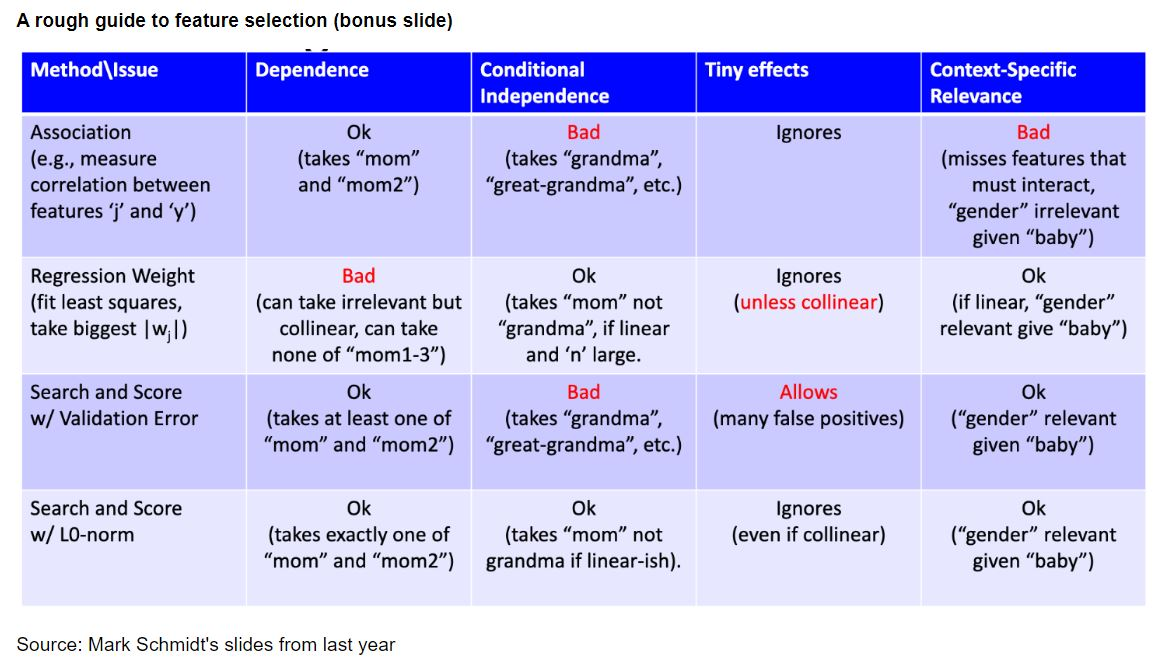
\includegraphics{C:/MyDisk/MDS/DSCI_571/FeatureSelect_summary.jpg}
\caption{FeatureSelect\_summary}
\end{figure}

\hypertarget{association-based-approaches-one-example-is-correlation}{%
\subsubsection{Association Based Approaches (one example is
correlation)}\label{association-based-approaches-one-example-is-correlation}}

\hypertarget{feature-ranking-with-recursive-feature-elimination.}{%
\paragraph{Feature ranking with Recursive Feature
Elimination.}\label{feature-ranking-with-recursive-feature-elimination.}}

\begin{itemize}
\tightlist
\item
  \href{https://scikit-learn.org/stable/modules/generated/sklearn.feature_selection.RFE.html\#sklearn.feature_selection.RFE}{sklearn.feature\_selection.RFE}
  (\texttt{sklearn.feature\_selection.RFE(estimator,\ n\_features\_to\_select=None,\ step=1,\ verbose=0)})
\item
  \href{https://scikit-learn.org/stable/modules/generated/sklearn.feature_selection.RFECV.html\#sklearn.feature_selection.RFECV}{Cross
  Validated
  RFE}(\texttt{sklearn.feature\_selection.RFECV(estimator,\ step=1,\ min\_features\_to\_select=1,\ cv=None,\ scoring=None,\ verbose=0,\ n\_jobs=None)})\\
\item
  Given an external estimator that assigns weights to features (e.g.,
  the coefficients of a linear model), the goal of recursive feature
  elimination (RFE) is to select features by recursively considering
  smaller and smaller sets of features.\\
\item
  First, the estimator is trained on the initial set of features and the
  importance of each feature is obtained either through a
  \texttt{coef\_} attribute or through a \texttt{feature\_importances\_}
  attribute.\\
\item
  Then, the least important features are pruned from current set of
  features. That procedure is recursively repeated on the pruned set
  until the desired number of features to select is eventually
  reached.\\
\item
  Allows NaN/Inf in the input if the underlying estimator does as well.
\end{itemize}

\begin{Shaded}
\begin{Highlighting}[]
\NormalTok{estimator }\OperatorTok{=}\NormalTok{ SVR(kernel}\OperatorTok{=}\StringTok{"linear"}\NormalTok{)}
\NormalTok{selector }\OperatorTok{=}\NormalTok{ RFE(estimator, }\DecValTok{5}\NormalTok{, step}\OperatorTok{=}\DecValTok{1}\NormalTok{)}
\NormalTok{selector }\OperatorTok{=}\NormalTok{ selector.fit(X, y)}
\NormalTok{selector.support_}
\NormalTok{selector.ranking_}
\end{Highlighting}
\end{Shaded}

\hypertarget{search-and-score-methods}{%
\subsubsection{Search and score
methods}\label{search-and-score-methods}}

\begin{itemize}
\tightlist
\item
  Most common feature selection framework

  \begin{itemize}
  \tightlist
  \item
    Define a \textbf{scoring function} \(f(S)\) that measures the
    quality of the set of features \(S\).\\
  \item
    Now \textbf{search} for the set of features \(S\) with the best
    score.\\
  \item
    Return \(S\) with the best score(lowest validation error).\\
  \end{itemize}
\item
  Problems

  \begin{itemize}
  \tightlist
  \item
    If there are \(d\) features, there are \(2^d\) combinations to
    search.\\
  \item
    Optimization bias is high: we are optimizing over \(2^d\) models!\\
  \item
    Prone to false positives: Irrelevant variables sometimes help by
    chance.
  \end{itemize}
\end{itemize}

A scoring function in score and search methods can be written as
follows.
\[ score(S) = \frac{1}{2}\lVert{Xw -y}\rVert^2 + \lambda \lVert w\rVert_0\]

\begin{itemize}
\tightlist
\item
  Here smaller \(\lVert w\rVert_0\) means we remove most of the
  features.

  \begin{itemize}
  \tightlist
  \item
    \textbf{Smaller \(\lVert w\rVert_0\) means we do not use many
    features.}\\
  \end{itemize}
\item
  And larger \(\lambda\) means aggressive feature selection.

  \begin{itemize}
  \tightlist
  \item
    \textbf{A larger \(\lambda\) means, we are forcing most of the
    weights to be 0 and so aggressive feature selection.}
  \end{itemize}
\item
  Hard to ``search'' because the search space is large.

  \begin{itemize}
  \tightlist
  \item
    \(2^d\) combinations to search if \(d\) is the number of features\\
  \end{itemize}
\item
  So instead of exhaustively searching for this space, we go with greedy
  approaches.
\end{itemize}

\hypertarget{forward-selectiongreedy-approach-not-implemented-in-sklearn-pseudo-code}{%
\paragraph{\texorpdfstring{Forward selection(Greedy approach, not
implemented in \texttt{sklearn}): Pseudo
code}{Forward selection(Greedy approach, not implemented in sklearn): Pseudo code}}\label{forward-selectiongreedy-approach-not-implemented-in-sklearn-pseudo-code}}

\begin{itemize}
\tightlist
\item
  Given \(X = \{x_1, x_2, \dots, x_n\}\) and \(y\)\\
\item
  Start with an empty set of features \(S = \{\}\)\\
\item
  Initialize the score (e.g., score = \(\infty\), if score is validation
  error)\\
\item
  For each possible feature \(x_j, 1\leq j \leq n\)

  \begin{itemize}
  \tightlist
  \item
    Compute the scores of features in \(S\) combined with \(x_j\)\\
  \end{itemize}
\item
  If no \(x_j\) improves the score, stop.\\
\item
  Otherwise add feature \(x_j\) to \(S\) which improves the score the
  most, update the score, and go back to step 2.\\
\item
  Not guaranteed to find the best feature set but reduces many problems

  \begin{itemize}
  \tightlist
  \item
    Cheaper (considers only \(O(d^2)\) models compared to \(O(2^d)\)
    models).\\
  \item
    Overfits less (less optimization bias).\\
  \item
    Reduces false positives (smaller chance of irrelevant variables
    helping by chance).
  \end{itemize}
\end{itemize}

\begin{quote}
There are some other types of stochastic search methods that inject
randomness so that we can explore new parts of the search space.
Example- Simulated annealing, Genetic algorithms, etc.
\end{quote}

\hypertarget{warnings-about-feature-selection}{%
\paragraph{Warnings about feature
selection}\label{warnings-about-feature-selection}}

\begin{itemize}
\tightlist
\item
  A feature is only relevant in the context of other features.

  \begin{itemize}
  \tightlist
  \item
    Adding/removing features can make features relevant/irrelevant.\\
  \end{itemize}
\item
  Confounding factors can make irrelevant features the most relevant.\\
\item
  If features can be predicted from other features, you cannot know
  which one to pick(Conditional independence).\\
\item
  Relevance for features does not have a causal relationship.
\end{itemize}

\hypertarget{general-advice-on-finding-relevant-features}{%
\paragraph{General advice on finding relevant
features}\label{general-advice-on-finding-relevant-features}}

\begin{itemize}
\tightlist
\item
  Try the association approach\\
\item
  Try forward selection with different values of \(\lambda\)\\
\item
  Try other feature selection methods (e.g., \texttt{RFE}, simulated
  annealing, genetic algorithms)\\
\item
  Talk to domain experts; they probably have an idea why certain
  features are relevant.
\end{itemize}

\hypertarget{performance-metrics}{%
\subsection{Performance Metrics}\label{performance-metrics}}

\begin{itemize}
\tightlist
\item
  \href{https://github.com/dariyasydykova/open_projects/tree/master/ROC_animation}{Awesome
  ROC Animations}
\item
  AUC tells us the area under an ROC curve, and, generally, an AUC value
  over 0.7 is indicative of a model that can distinguish between the two
  outcomes well. An AUC of 0.5 tells us that the model is a random
  classifier, and it cannot distinguish between the two outcomes. The
  shape of an ROC curve changes when a model changes the way it
  classifies the two outcomes.\\
\item
  Precision-recall curve also displays how well a model can classify
  binary outcomes. Similarly to the ROC curve, when the two outcomes
  separate, precision-recall curve will approach the top-right corner.
  Typically, a model that produces a precision-recall curve that is
  closer to the top-right corner is better than a model that produces a
  precision-recall curve that is skewed towards the bottom of the
  plot.\\
\item
  Precision-recall curve is more sensitive to class imbalanace than an
  ROC curve. ROC curve tends to be more robust to class imbalanace that
  a precision-recall curve.\\
\item
  When the standard deviation of one of the outcomes changes, an ROC
  curve and its AUC value also change.\\
\item
  It might indicate that the model performance has increased, when, in
  fact, the prediction performance has worsened for e.g.~at small false
  positive rates.\\
\item
  My Understanding of the ROC curve: In a perfect model:

  \begin{itemize}
  \tightlist
  \item
    When everything is classified as 1 (the probability threshold is 0)
    then TPR is 1 \& FPR is also 1.\\
  \item
    When we increase the threshold then TPR stays at 1 \& FPR
    decreases.\\
  \item
    At a point when TPR is still 1 \& FPR becomes 0 then we are
    classifying exactly the same number of 1s as the data has.\\
  \item
    Beyond that point FPR stays at 0 \& TPR decreases until we are
    classifying no 1s \& TPR also becomes 0.\\
  \item
    This describes a perfect shape of the ROC curve. For an imperfect
    model the shape is distorted but is similar to ideal shape.
  \end{itemize}
\end{itemize}

\hypertarget{regularization}{%
\subsection{Regularization}\label{regularization}}

\textbf{How to pick \(\lambda\)?:}

\begin{itemize}
\tightlist
\item
  Theory: as \(n\) grows \(\lambda\) should be in the range \(O(1)\) to
  \(\sqrt{n}\).
\item
  Practice: optimize validation set or cross-validation error.
\end{itemize}

\hypertarget{l0-penalty}{%
\subsubsection{L0 Penalty}\label{l0-penalty}}

\[ score(S) = \frac{1}{2}\lVert{Xw -y}\rVert^2 + \lambda \lVert w\rVert_0\]

\hypertarget{l2-regularization}{%
\subsubsection{L2 regularization}\label{l2-regularization}}

\begin{itemize}
\item
  \texttt{sklearn.linear\_model.Ridge}: Ridge regression addresses some
  of the problems of Ordinary Least Squares by imposing a penalty on the
  size of the coefficients with l2 regularization.
\item
  \texttt{class\ sklearn.linear\_model.Ridge(alpha=1.0,\ fit\_intercept=True,\ normalize=False,\ copy\_X=True,\ max\_iter=None,\ tol=0.001,\ solver=\textquotesingle{}auto\textquotesingle{},\ random\_state=None)}
\item
  Standard regularization strategy is L2-regularization

  \begin{itemize}
  \tightlist
  \item
    \(\lambda \rightarrow\) regularization strength
  \item
    \(\lVert w\rVert_2^2 \rightarrow\) \(L2\) norm of \(w\)

    \begin{itemize}
    \tightlist
    \item
      square root of the sum of the squared weight values.
    \end{itemize}
  \end{itemize}
\end{itemize}

\[f(w) = \frac{1}{2}\sum_i^n(w^TX_i - y_i)^2 + \frac{\lambda}{2}\sum_j^d w_j^2 \text{ or }\]
\[f(w) = \frac{1}{2}\lVert Xw - y\rVert_2^2 + \frac{\lambda}{2} \lVert w\rVert_2^2\]

\begin{itemize}
\tightlist
\item
  Balances getting low error vs.~having small slopes \(w_j\)
\item
  In terms of fundamental trade-off:

  \begin{itemize}
  \tightlist
  \item
    You can increase the training error if it makes \(w\) much smaller.
  \item
    Nearly-always reduces overfitting.
  \end{itemize}
\item
  Penalizing \(w_j^2\) means different things if features \(j\) are on
  different scales. So Scaling is important in this case.
\item
  \(\lVert Xw - y\rVert^2\) increases with \(\lambda\), and
  \(\lVert w\rVert^2\) decreases with λ.

  \begin{itemize}
  \tightlist
  \item
    Though individual \(w_j\) can increase or decrease with lambda
    because we use the L2-norm, the large ones decrease the most.
  \end{itemize}
\end{itemize}

\begin{quote}
\textbf{Should we regularize the y-intercept?}
\end{quote}

\begin{itemize}
\tightlist
\item
  No!: Why encourage it to be closer to zero? (It could be anywhere.).
  You should be allowed to shift function up/down globally.
\item
  Yes!: It makes the solution unique and it easier to compute \(w\).
\item
  Compromise: regularize by a smaller amount than other variables.

  \begin{itemize}
  \tightlist
  \item
    \(f(w) = \lVert Xw + w_0 - y\rVert^2 + \frac{\lambda}{2}\lVert w\rVert^2 + \frac{\lambda}{2}w_0^2\)
  \end{itemize}
\end{itemize}

\begin{quote}
\textbf{Some properties of L2 regularization}
\end{quote}

\begin{itemize}
\tightlist
\item
  Solution \(w\) is unique and fast.
\item
  Almost always improves the validation error.
\item
  No collinearity issues.
\item
  Less sensitive to changes in \(X\) or \(y\).
\item
  Gradient descent converges faster (bigger \(\lambda\) means fewer
  iterations).
\item
  Worst case: just set \(\lambda\) small and get the same performance.
\end{itemize}

\hypertarget{l1-regularization}{%
\subsubsection{L1 regularization}\label{l1-regularization}}

\begin{itemize}
\tightlist
\item
  \texttt{sklearn.linear\_model.Lasso}: The Lasso is a linear model that
  estimates sparse coefficients with l1 regularization.
\end{itemize}

\hypertarget{dealing-with-data-imbalance-model-explainers}{%
\subsection{Dealing with data imbalance, model
explainers}\label{dealing-with-data-imbalance-model-explainers}}

\begin{Shaded}
\begin{Highlighting}[]
\NormalTok{X_adult,y_adult }\OperatorTok{=}\NormalTok{ shap.datasets.adult()}
\NormalTok{X_adult_display,y_adult_display }\OperatorTok{=}\NormalTok{ shap.datasets.adult(display}\OperatorTok{=}\VariableTok{True}\NormalTok{)}
\NormalTok{X_adult_train, X_adult_test, y_adult_train, y_adult_test }\OperatorTok{=}\NormalTok{ train_test_split(X_adult, y_adult, test_size }\OperatorTok{=} \FloatTok{0.2}\NormalTok{, random_state }\OperatorTok{=} \DecValTok{111}\NormalTok{)}
\NormalTok{X_adult_display.head(}\DecValTok{5}\NormalTok{)}
\end{Highlighting}
\end{Shaded}

\hypertarget{approaches-to-handle-class-imbalance}{%
\subsubsection{Approaches to handle Class
Imbalance}\label{approaches-to-handle-class-imbalance}}

\begin{itemize}
\item
  \texttt{class\_weight} (dict, `balanced' or None) parameter of many
  scikit learn algorithms is used to provide weights associated with
  classes in the form \texttt{\{class\_label:\ weight\}}. If not given,
  all classes are supposed to have weight one.

  \begin{itemize}
  \tightlist
  \item
    This was equivalent to saying ``repeat every positive example
    \texttt{weight} number of times in the training set''.
  \item
    \texttt{class\_weight="balanced"}: This sets the weights so that the
    classes are ``equal''. The ``balanced'' mode uses the values of y to
    automatically adjust weights inversely proportional to class
    frequencies in the input data as n\_samples / (n\_classes *
    np.bincount(y)).
  \item
    \texttt{sklearn.utils.class\_weight.compute\_class\_weight(\textquotesingle{}balanced\textquotesingle{},\ classes,\ y)}:
    This can be used to calculate weights used by sklearn using the
    balanced method.
  \item
    changing the class weight will \textbf{generally reduce accuracy}.
    The original model was trying to maximize accuracy.
  \end{itemize}
\item
  \textbf{Undersampling}: Take a random sample from the majority class
  of size equal to the minority class.

  \begin{itemize}
  \tightlist
  \item
    This is generally not considered a good approach.
  \end{itemize}
\item
  \textbf{Random oversampling of the minority class with replacement}
\item
  \textbf{SMOTE (Synthetic Minority Over-sampling Technique)}

  \begin{itemize}
  \tightlist
  \item
    Create ``synthetic'' examples rather than by over-sampling with
    replacement.
  \item
    The minority class is over-sampled by taking each minority class
    sample and introducing synthetic examples along the line segments
    joining any/all of the \(k\) minority class nearest neighbors.
  \item
    \(k\) is chosen depending upon the amount of over-sampling required.
  \item
    Take the difference between the feature vector (sample) under
    consideration and its nearest neighbor.
  \item
    Multiply this difference by a random number between 0 and 1, and add
    it to the feature vector under consideration.
  \item
    This causes the selection of a random point along the line segment
    between two specific features.
  \item
    This approach effectively forces the decision region of the minority
    class to become more general.
  \end{itemize}
\end{itemize}

\begin{Shaded}
\begin{Highlighting}[]
\CommentTok{# Let's try to create samples using SMOTE}
\NormalTok{sm }\OperatorTok{=}\NormalTok{ SMOTE(random_state}\OperatorTok{=}\DecValTok{42}\NormalTok{)}
\NormalTok{X_train_sm, y_train_sm }\OperatorTok{=}\NormalTok{ sm.fit_resample(X_train, y_train)}
\NormalTok{smote_model }\OperatorTok{=}\NormalTok{ LogisticRegression(solver }\OperatorTok{=} \StringTok{'liblinear'}\NormalTok{, max_iter}\OperatorTok{=}\DecValTok{500}\NormalTok{)}
\NormalTok{smote_model.fit(X_train_sm, y_train_sm)}\OperatorTok{;}

\CommentTok{### sklearn Pipeline won't work here}
\CommentTok{### So let's use imblearn.pipeline}
\ImportTok{from}\NormalTok{ imblearn.pipeline }\ImportTok{import}\NormalTok{ Pipeline}
\NormalTok{pipe }\OperatorTok{=}\NormalTok{ Pipeline(steps}\OperatorTok{=}\NormalTok{[(}\StringTok{'smote'}\NormalTok{, SMOTE()),}
\NormalTok{                       (}\StringTok{'classifier'}\NormalTok{, LogisticRegression(solver }\OperatorTok{=} \StringTok{'liblinear'}\NormalTok{, max_iter}\OperatorTok{=}\DecValTok{500}\NormalTok{))])}
\NormalTok{weights }\OperatorTok{=}\NormalTok{ np.linspace(}\FloatTok{0.05}\NormalTok{, }\FloatTok{0.95}\NormalTok{, }\DecValTok{20}\NormalTok{)}
\NormalTok{param_grid}\OperatorTok{=}\NormalTok{\{}
    \StringTok{'smote__sampling_strategy'}\NormalTok{: weights}
\NormalTok{\}}

\NormalTok{gs }\OperatorTok{=}\NormalTok{ GridSearchCV(estimator}\OperatorTok{=}\NormalTok{pipe,  }
\NormalTok{                  param_grid }\OperatorTok{=}\NormalTok{ param_grid, }
\NormalTok{                  scoring}\OperatorTok{=}\StringTok{'f1'}\NormalTok{,}
\NormalTok{                  cv}\OperatorTok{=}\DecValTok{5}\NormalTok{,}
\NormalTok{                  return_train_score }\OperatorTok{=} \VariableTok{True}
\NormalTok{                 )}
\NormalTok{gs.fit(X_train, y_train)}\OperatorTok{;}
\end{Highlighting}
\end{Shaded}

\hypertarget{stratified-sampling}{%
\subsubsection{Stratified Sampling}\label{stratified-sampling}}

\begin{itemize}
\tightlist
\item
  A similar idea of ``balancing'' classes can be applied to data splits.
\item
  \href{https://scikit-learn.org/stable/modules/generated/sklearn.model_selection.StratifiedKFold.html}{\texttt{StratifiedKFold}}:
  This cross-validation object is a variation of KFold that returns
  stratified folds. The folds are made by preserving the percentage of
  samples for each class.
\item
  For e.g.~if we have 10\% negative examples in total, then each fold
  will have 10\% negative examples.
\item
  We have the same option in \texttt{train\_test\_split} with the
  \texttt{stratify} argument.
\item
  Since its no longer a random sample, probably theoretically bad, but
  not that big of a deal.
\item
  It can be especially useful in multi-class, say if you have one class
  with very few cases.
\end{itemize}

\hypertarget{model-interpretability}{%
\subsection{Model Interpretability}\label{model-interpretability}}

\hypertarget{eli5}{%
\subsubsection{\texorpdfstring{\href{https://eli5.readthedocs.io/en/latest/tutorials/black-box-text-classifiers.html\#lime-tutorial}{eli5}}{eli5}}\label{eli5}}

ELI5 is a Python library which allows to visualize and debug various
Machine Learning models using unified API. It has built-in support for
several ML frameworks and provides a way to explain black-box models.

\begin{Shaded}
\begin{Highlighting}[]
\NormalTok{X,y }\OperatorTok{=}\NormalTok{ shap.datasets.adult()}
\NormalTok{X_display,y_display }\OperatorTok{=}\NormalTok{ shap.datasets.adult(display}\OperatorTok{=}\VariableTok{True}\NormalTok{)}

\CommentTok{### How to look at weights if you have transformed the data}
\NormalTok{marital_status_feature }\OperatorTok{=}\NormalTok{ [}\StringTok{'Marital Status'}\NormalTok{]}
\NormalTok{other_features }\OperatorTok{=}\NormalTok{ [}\StringTok{'Age'}\NormalTok{, }\StringTok{'Workclass'}\NormalTok{, }\StringTok{'Education-Num'}\NormalTok{, }\StringTok{'Occupation'}\NormalTok{,}
       \StringTok{'Relationship'}\NormalTok{, }\StringTok{'Race'}\NormalTok{, }\StringTok{'Sex'}\NormalTok{, }\StringTok{'Capital Gain'}\NormalTok{, }\StringTok{'Capital Loss'}\NormalTok{,}
       \StringTok{'Hours per week'}\NormalTok{, }\StringTok{'Country'}\NormalTok{]}

\NormalTok{marital_status_transformer }\OperatorTok{=}\NormalTok{ Pipeline(steps}\OperatorTok{=}\NormalTok{[}
\NormalTok{                                          (}\StringTok{'onehot'}\NormalTok{, OneHotEncoder(sparse}\OperatorTok{=}\VariableTok{False}\NormalTok{, handle_unknown}\OperatorTok{=}\StringTok{'ignore'}\NormalTok{))}
\NormalTok{                                         ])}

\NormalTok{preprocessor }\OperatorTok{=}\NormalTok{ ColumnTransformer(}
\NormalTok{                                 transformers}\OperatorTok{=}\NormalTok{[}
\NormalTok{                                    (}\StringTok{'marital'}\NormalTok{, marital_status_transformer, marital_status_feature),}
\NormalTok{                                    (}\StringTok{'other'}\NormalTok{, }\StringTok{"passthrough"}\NormalTok{, other_features)}
\NormalTok{                                ])}

\NormalTok{xgb }\OperatorTok{=}\NormalTok{ XGBClassifier()}
\NormalTok{xgb_ppl }\OperatorTok{=}\NormalTok{ Pipeline(steps}\OperatorTok{=}\NormalTok{[(}\StringTok{'preprocessor'}\NormalTok{, preprocessor),}
\NormalTok{                      (}\StringTok{'classifier'}\NormalTok{, xgb)])}
\NormalTok{xgb_ppl.fit(X, y)}\OperatorTok{;}
\NormalTok{ohe_features }\OperatorTok{=}\NormalTok{ xgb_ppl[}\StringTok{'preprocessor'}\NormalTok{].transformers_[}\DecValTok{0}\NormalTok{][}\DecValTok{1}\NormalTok{][}\StringTok{'onehot'}\NormalTok{].get_feature_names(marital_status_feature)}
\NormalTok{all_features }\OperatorTok{=}\NormalTok{ other_features }\OperatorTok{+} \BuiltInTok{list}\NormalTok{(ohe_features)}

\NormalTok{eli5.explain_weights(xgb_ppl[}\StringTok{'classifier'}\NormalTok{], feature_names }\OperatorTok{=}\NormalTok{ all_features)}
\end{Highlighting}
\end{Shaded}

\hypertarget{shap}{%
\subsubsection{\texorpdfstring{\href{https://github.com/vermashivam679/shap}{SHAP}}{SHAP}}\label{shap}}

\begin{itemize}
\tightlist
\item
  Calculates \textbf{SHAP} values, which are rooted in game theory, as a
  unified measure of feature importance.
\item
  \emph{Provides following kind of explanation}: Start at a base rate
  (e.g., how often people get their loans rejected). Add one feature at
  a time and see how it impacts the decision.
\item
  The order of the features we consider matters!
\item
  In cooperative games find each player's marginal contribution,
  averaged over every possible sequence in which the players could have
  been added to the group.
\item
  Computationally challenging, SHAP provides an efficient way to deal
  with this.
\end{itemize}

Provides explainer for different kinds of models

\begin{itemize}
\tightlist
\item
  \href{https://shap.readthedocs.io/en/latest/}{TreeExplainer} (supports
  XGBoost, CatBoost, LightGBM)
\item
  \href{https://shap.readthedocs.io/en/latest/index.html\#shap.DeepExplainer}{DeepExplainer}
  (supports deep-learning models)
\item
  \href{https://shap.readthedocs.io/en/latest/index.html\#shap.KernelExplainer}{KernelExplainer}
  (supports kernel-based models)
\item
  \href{https://shap.readthedocs.io/en/latest/index.html\#shap.GradientExplainer}{GradientExplainer}
  (supports Keras and Tensorflow models)
\end{itemize}


\end{document}
